
\documentclass[a4paper]{article}

\usepackage[T1]{fontenc}
\usepackage[swedish]{babel}
\usepackage[utf8]{inputenc}
\usepackage{amsmath}
\usepackage{amssymb}
\usepackage{fancyhdr}
\usepackage{tikz}
\usetikzlibrary{decorations.pathmorphing,shapes,arrows,positioning,calc}
\usepackage[hidelinks]{hyperref}


\newcommand{\coursecode}{ERE102}
\newcommand{\coursename}{Reglerteknik D}
\newcommand{\doctitle}{Tentalösningar}

\newcommand{\mhb}[1]{$\beta_{\text{#1}}$}     % Mathematics Handbook Beta
\newcommand{\bl}[1]{$\text{BL}_{\text{#1}}$}  % Bengt Lennartsson



%--------grstep
% For denoting a Gauss' reduction step.
% Use as: \grstep{\rho_1+\rho_3} or \grstep[2\rho_5 \\ 3\rho_6]{\rho_1+\rho_3}
% \newcommand{\grstep}[2][\relax]{%
%    \ensuremath{\mathrel{
%        \mathop{\longrightarrow}\limits^{#2\mathstrut}_{
%                                    \begin{subarray}{l} #1 \end{subarray}}}}}

% Advantage of length formulation is that between adjacent
% \grstep's you can add \hspace{-\grsteplength} to make it look not too wide
\newlength{\grsteplength}
\setlength{\grsteplength}{1.5ex plus .1ex minus .1ex}

\newcommand{\grstep}[2][\relax]{%
   \ensuremath{\mathrel{
       \hspace{\grsteplength}\mathop{\longrightarrow}\limits^{#2\mathstrut}_{
                                     \begin{subarray}{l} #1 \end{subarray}}\hspace{\grsteplength}}}}
% If two or more \grsteps are in a row then they need to be tightened
\newcommand{\repeatedgrstep}[2][\relax]{\hspace{-\grsteplength}\grstep[#1]{#2}}

% row swap operation: \rho_1\swap\rho_2
\newcommand{\swap}{\leftrightarrow}



\newenvironment{amat}[2][c]{%
  % disable optional arg \left(\begin{array}{@{}*{#2}{#1}|#1@{}}
  \left[\begin{array}{@{}*{#2}{c}|#1@{}}
}{%
  \end{array}\right]
}


\newcommand{\oklarhet}[1]{%
  \noindent\fbox{\parbox[b][4em][t]{\textwidth}{\color{red}#1} }%
}


\tikzset{
block/.style = {draw, fill=white, rectangle, minimum height=3em, minimum width=3em},
tmp/.style  = {coordinate},
sum/.style= {draw, fill=white, circle, node distance=1cm},
input/.style = {coordinate},
output/.style= {coordinate},
pinstyle/.style = {pin edge={to-,thin,black}
}
}



\pagestyle{fancy}
\topmargin -20.0pt
\headheight 56.0pt
\rhead{
  \coursename\\
  \doctitle
}
\setlength{\topskip}{0pt} % Skip some whitespace at the top
\newcommand{\horrule}[1]{\rule{\linewidth}{#1}} % Create horizontal rule command with 1 argument of height





\begin{document}
\thispagestyle{plain} % No header for first page


\begin{center}
\horrule{0.5pt} \\[0.3cm] % Thin top horizontal rule
%
\huge  \coursecode -- \coursename \\[1mm]
\Large \doctitle
\normalsize % Revert to normal sized font

\horrule{2pt} \\[0.1cm] % Thick bottom horizontal rule

\begin{tabular}{ l r }
  Av Johan Sjöblom & sjoblomj88@gmail.com
\end{tabular}\\[0.1cm]
\footnotesize Version: 1.0, Augusti 2014\\[0.4cm]

\end{center}
{\footnotesize
Please feel free to spread the document to anyone that wants it, and please improve the solutions if you can. All of the document, as well as the \LaTeX{} code, is public domain.

Note! These solutions are not from the department giving the course, and they have not been checked for errors. The answers might not be explicit enough to give full points.\\
}
\horrule{0.5pt} % Thin top horizontal rule
\normalsize % Revert to normal sized font
\\[2.5cm]

\resizebox{!}{120mm}
{
\includegraphics{p1110461.jpg}}

\begin{tikzpicture}[overlay,remember picture]
    \pgftransformshift{\pgfpointanchor{current page}{center}}
    \node[
        ellipse callout,
        draw=red,
        ultra thick,
        fill=yellow,
        callout relative pointer=(245:1cm),
        font=\Huge,
        text width=0.4\textwidth,
        align=center,
        anchor=center
        ] at (2,2) {Jag har klarat regleren};
\end{tikzpicture}

%\section{Tenta 2012-12-21}
%\subsection{1a}
%Löst.
%
%
%\subsection{1b}
%Sida 42. har foto på't.
%
%
%\subsection{1d}
%Foto på halva.



\section{Tenta 2014-04-24}
\subsection{1a}
\begin{align*}
  \ddot{y}(t) + \dot{y}(t) = u(t - 1)
\end{align*}
Notera att uppgiften säger att $u$ är insignal, och alltså inte ett steg!
%
Laplacea med hjälp av \mhb{L8} ($\ddot{y}(t)$), \mhb{L7} ($\dot{y}(t)$) och \mhb{L4} ($u(t - 1)$):
\begin{align*}
  s^2Y(s) + sY(s) = e^{-1 \cdot s}U(s) \\
  Y(s)(s^2 + s) = U(s)e^{-s}
\end{align*}
Överföringsfunktionen blir:
\begin{align*}
  G(s) = \frac{Y(s)}{U(s)} = \frac{e^{-s}}{s^2 + s}
\end{align*}

Detta är inte ett trevligt problem; tidsförskjutningen (alltså $u(t-1)$ i den givna ekvationen) ger upphov till $e^{-s}$, vilket gör det hela besvärligt att arbeta med. Vi struntar tillsvidare i tidsförskjutningen, och kompenserar för det i efterhand. Detta kan vi göra om systemet är tidsinvariant, vilket alla system i Reglerteknikkursen är. Om vi alltså istället för att räkna på den givna ekvationen tittar på följande,
\begin{align*}
  \ddot{y}(t) + \dot{y}(t) = u(t)
\end{align*}
så får vi på samma sätt som ovan:
\begin{align*}
  s^2Y(s) + sY(s) = U(s) \\
  Y(s)(s^2 + s) = U(s)
\end{align*}
%
Överföringsfunktionen, (nu kallad $G_{\text{ny}}(s)$, då det ju inte är samma som vi tidigare hade) blir:
\begin{align*}
  G_{\text{ny}}(s) = \frac{Y(s)}{U(s)} = \frac{1}{s^2 + s}
\end{align*}
%
Vi vill bestämma systemets stegsvar, det vill säga $y(t)$ då insignalen är ett steg. Det får vi genom att invers-Laplacea $Y(s)$. Ett steg i Laplacedomänen innebär att insignalen $U(s) = \frac{1}{s}$. Vi har $G_{\text{ny}}(s)$ och $U(s)$, och vill ha ut $Y(s)$. Detta ger:
\begin{align*}
  G_{\text{ny}}(s) = \frac{Y(s)}{U(s)} \Longleftrightarrow Y(s) = G_{\text{ny}}(s)U(s) = \frac{1}{s^2 + s} \cdot \frac{1}{s} = \frac{1}{s^2(s + 1)}
\end{align*}
%
För att lösa detta använder vi oss av partialbråksuppdelning (se sektion \ref{sec:partialbråksuppdelning}).
%
\begin{align*}
  Y(s) &= \frac{1}{s^2(s + 1)} = \frac{A}{s^2} + \frac{B}{s} + \frac{C}{s+1} \Longleftrightarrow \\
  1 &= A(s + 1) + Bs(s + 1) + Cs^2 \Longleftrightarrow \\
  1 &= As + A + Bs^2 + Bs + Cs^2
\end{align*}
%
Vi skiljer på gradtalen:
%
\begin{align*}
  s^2: & \quad B + C = 0\\
  s^1: & \quad A + B = 0\\
  s^0: & \quad A     = 1
\end{align*}
%
Detta kan lösas på flera sätt, till exempel genom att sätta upp på matrisform:
%
\begin{equation*}
    \begin{amat}[r]{3}
      1  &0  &0  &1  \\
      1  &1  &0  &0  \\
      0  &1  &1  &0
    \end{amat}
  \grstep{-\rho_1 +\rho_2}
  \begin{amat}[r]{3}
       1  &0  &0  &1  \\
       0  &1  &0  &-1 \\
       0  &1  &1  &0
     \end{amat}
  \grstep{-\rho_2 +\rho_3}
  \begin{amat}[r]{3}
       1  &0  &0  &1  \\
       0  &1  &0  &-1 \\
       0  &0  &1  &1
     \end{amat}
\end{equation*}
Vi får alltså:
\begin{align*}
  \begin{cases}
    A = 1 \\
    B = -1 \\
    C = 1
  \end{cases}
\end{align*}
%
Stoppar vi in värdena i $Y(s)$ så får vi:
\begin{align*}
  Y(s) = G_{\text{ny}}(s)U(s) = \frac{1}{s^2(s + 1)} = \frac{A}{s^2} + \frac{B}{s} + \frac{C}{s+1} = \frac{1}{s^2} - \frac{1}{s} + \frac{1}{s+1}
\end{align*}
%
Detta kan vi enkelt invers-Laplacea med hjälp av \mhb{L20} ($\frac{1}{s^2}$), \mhb{L18} ($\frac{1}{s}$) och \mhb{L21} ($\frac{1}{s+1}$).
%
\begin{align*}
  y(t) = t^1 - 1 + e^{-1\cdot t} = t - 1 + e^{-t}, \qquad t \geq 0 \quad (y(t) = 0, t < 0)
\end{align*}
%
Detta har vi alltså löst då vi struntat i den tidsfördröjning som fanns med i ursprungsproblemet (det vill säga vi har förbisett att differentialekvationen innehöll termen $u(t-1)$ och istället räknat på $u(t)$). Då fördröjningen är 1 tidsenhet, så ersätter vi $t$ i resultatet med $t-1$:
\begin{align*}
  y(t) = (t - 1) - 1 + e^{-(t - 1)} = t - 2 + e^{-t + 1}, \qquad t \geq 1 \quad (y(t) = 0, t < 1)
\end{align*}



\subsection{1b}
Teorin bakom detta står på \bl{sid 424}.\\\\
%
Vi ska bestämma en tillståndsåterkoppling. Med andra ord så har vi ett öppet system, och ska återkoppla det.\\
%
I det allmänna fallet så gäller
\begin{align*}
  \dot{x}(t) =~& Ax(t) + Bu(t) \\
  y(t) =~& Cx(t) + Du(t)
\end{align*}
och i vårt fall så har vi
\begin{align*}
  \dot{x}(t) =& \begin{bmatrix}-4 & -3 \\ 1 & 0\end{bmatrix} x(t) + \begin{bmatrix}1 \\ 0\end{bmatrix} u(t) \\
  y(t) =& \begin{bmatrix}1 & 1\end{bmatrix} x(t)
\end{align*}
%
%
Då vi har ett öppet system så kan vi enligt ekvation 3.15 på \bl{sid 92} räkna ut polerna med $\det(sI-A) = 0$ (om det var ett slutet system så hade (11.15) på \bl{sid 425} gällt). Hur man räknar ut determinanter står på \mhb{sid 93}.
%
\begin{align*}
  \det(sI-A) = 0 \Longleftrightarrow \\
  0 = \det \left( \begin{bmatrix}s & 0 \\ 0 & s\end{bmatrix} - \begin{bmatrix}-4 & -3 \\ 1 & 0\end{bmatrix} \right) = \det \left( \begin{bmatrix}s+4 & 3 \\ -1 & s\end{bmatrix} \right) =\\
  (s+4)s - 3(-1) = s^2 + 4s + 3 = 0\\
  s=-\frac{4}{2} \pm \sqrt{\left(\frac{4}{2}\right)^2 - 3}\\
  s=-2 \pm 1\\
  s_1=-3, \qquad s_2=-1\\
\end{align*}
%
%
\oklarhet{Referens till polavstånd vs. hastighet på systemet?}\\
Ökat avstånd till origo ger snabbare system. Den långsamma polen är alltså $s_2=-1$. Detta innebär att vi vill placera den långsamma polen $s_2$ i den snabba polen $s_1$. Alltså sätter vi att $s_1 = s_2 = -3$. Har vi båda polerna i $-3$ så blir den karakteristiska ekvationen $\alpha_c(s) = (s+3)^2 = s^2 + 6s + 9$.\\\\
%
%
Enligt (11.15) på \bl{sid 425} så gäller att när vi ``uttrycker den önskade polplaceringen för det återkopplade systemet i form av det karakteristiska polynomet ($\alpha_c(s)$), leder det till att följande polynomidentitet ska uppfyllas: $\alpha_c(s) = \det(sI -A + BL_u)$''. Med andra ord, den karakteristiska ekvationen vi nyss räknade ut ska vara lika med $\det(sI -A + BL)$.
%
\begin{align*}
  \det(s I - A + BL) = \det\left(\begin{bmatrix}s & 0 \\ 0 & s \end{bmatrix} - \begin{bmatrix}-4 & -3 \\ 1 & 0\end{bmatrix} + \begin{bmatrix}1 \\ 0\end{bmatrix} \begin{bmatrix}l_1 & l_2\end{bmatrix} \right) = \\
  \det \left(\begin{bmatrix}s+4 & 3 \\ -1 & s \end{bmatrix} + \begin{bmatrix}l_1 & l_2 \\ 0 & 0\end{bmatrix} \right) = \det \left(\begin{bmatrix}s+4+l_1 & 3+l_2 \\ -1 & s\end{bmatrix} \right) = \\
  (s+4+l_1)s - (3+l_2)(-1) = \\
  s^2 +4s + l_1s + 3 + l_2 = s^2 + (4+l_1)s + (3 + l_2)
\end{align*}
%
Detta är alltså enligt (11.15) lika med den karakteristiska ekvationen ($\alpha_c(s)$), varifrån vi kan identifiera värden på $l_1$ och $l_2$:
%
\begin{eqnarray*}
  s^2 + &(4+l_1)s &+ (3 + l_2) = \\
  s^2 + &6s &+ 9\\
\end{eqnarray*}
\vspace{-14mm}
\begin{align*}
  \left\{ \begin{array}{ll}
  4+l_1 = 6\\
  3+l_2 = 9
  \end{array} \right. \Longleftrightarrow
  \left\{ \begin{array}{ll}
  l_1 = 2\\
  l_2 = 6
  \end{array} \right.
\end{align*}


\subsection{1d}
Från bifogat formelblad till tesen:\\
%
LP $\rightarrow$ HP: $\qquad s \rightarrow \frac{\omega_c}{s}$.\\\\
%
%
På något sätt så ser vi att när vi utgår från första ordningens Butterworth-filter, så har vi\\
\oklarhet{Hur ser vi detta?}
%
\begin{align*}
  |H(i\omega)|^2 = \frac{1}{1 + (\frac{\omega}{\omega_c})^{2n}}
\end{align*}
%
Nu har vi\\
\oklarhet{Hur?}
\begin{align*}
  H(s) = \frac{1}{1 + \underbrace{s}_{s \rightarrow \frac{\omega_c}{s}}} \rightarrow \frac{1}{1 + \frac{\omega_c}{s}} = \frac{s}{\omega_c + s}
\end{align*}
%
Från bifogat formelblad till tesen så har vi att Tustin-diskretisering innebär:
\begin{align*}
  s \rightarrow \frac{2}{h} \frac{1 - z^{-1}}{1 + z ^{-1}} = \frac{2}{h} \frac{1 - \frac{1}{z}}{1 + \frac{1}{z}} = \frac{2}{h} \frac{z - 1}{z + 1}
\end{align*}
%
Om vi Tustin-diskretiserar $H(s)$ så får vi:
\begin{align*}
  H(z) = \frac{\frac{2}{h} \frac{z - 1}{z + 1}}{\omega_c + \frac{2}{h} \frac{z - 1}{z + 1}} = \frac{2(z - 1)}{\omega_c h (z+1) + 2(z-1)} = \frac{z-1}{z-1 + \frac{1}{2} \omega_c h (z+1)}
\end{align*}

På något sätt så ser vi att $\omega_c = 2\pi \cdot 500$ Hz. Vi ljuger oss också till att $h$ är angivet i sekunder, och att $h = 10^4 \text{ Hz} \Rightarrow (10^4)^{-1}$. Sätter vi in det så får vi:\\
\oklarhet{Hur gick det till?}
%
\begin{align*}
  H(z) = \frac{z-1}{z-1 + \frac{1}{2} 2\pi 500 \cdot (10^4)^{-1} (z+1)} = \frac{z-1}{z-1 + 0.05 \pi (z+1)} = \\
  \frac{z-1}{(0.05\pi + 1)z + 0.05 \pi -1} = \frac{\frac{1}{(0.05\pi + 1)}(z-1)}{z + \frac{0.05 \pi -1}{(0.05\pi + 1)}} \approx \frac{0.86(z-1)}{z-0.73}\\
\end{align*}

\section{Tenta 2013-12-16}
\subsection{1a}
Ett insignal-utsignal-stabilt system har sina poler strikt i vänster halvplan. Vi vill alltså hitta polerna och kontrollera vart de ligger, för att avgöra om systemen är stabila eller inte. Polerna hittar vi genom att sätta nämnarna i ekvationerna till 0, och sedan lösa ut $s$.

\begin{align*}
  G_1(s) = \frac{s-3}{s^2+2s+6}
\end{align*}
%
Sätt nämnaren till 0 och lös:
\begin{align*}
  s^2+2s+6 = 0\\
  s = -\frac{2}{2} \pm \sqrt{\left(\frac{2}{2}\right)^2 -6}\\
  s = -1 \pm \sqrt{-5}\\
  s_1 = -1 + 5i, \qquad s_2 = -1 - 5i
\end{align*}
%
Vi ser att båda polerna har imaginära delar, men det spelar ingen roll. Det viktiga är att båda ligger i vänster halvplan, vilket de ju gör. $G_1(s)$ är alltså stabilt.

\begin{align*}
  G_2(s) = \frac{s+3}{s^2+2s} = \frac{s+3}{s(s+2)}
\end{align*}
%
Polerna får vi alltså av $s(s+2) = 0$. Vi ser omedelbart att $s_1 = -2$ och $s_2 = 0$. Polen $s_1$ ligger i vänster halvplan, men $s_2$ ligger på 0, och alltså inte strikt i vänster halvplan. $G_2(s)$ är alltså inte stabilt.


\subsection{1b}
Vi ska bestämma överföringsfunktionen från $\theta_i$ till $\theta_0$. Gyroåterkopplingen subtraherar $\theta_0Ks$ från insignalen, men givet i uppgiften är att $K=0$, vilket alltså gör att gyroåterkopplingen faller bort. Blockdiagrammet reduceras till följande:\\
%
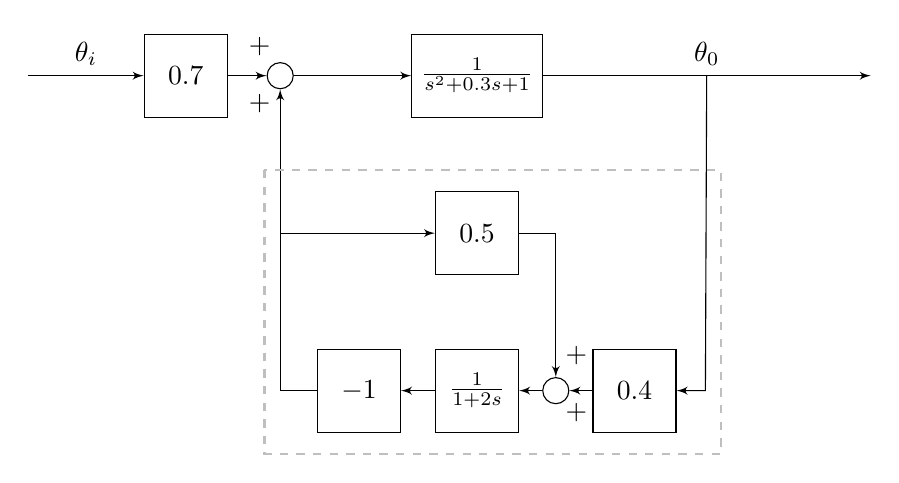
\begin{tikzpicture}[auto, node distance=2cm,>=latex']
  \node [input, name=rinput]                            (rinput)    {};
  \node [block, right of=rinput]                        (block07)   {$0.7$};
  \node [sum, right of=block07, node distance=1.2cm]    (suma)      {};
  \node [tmp, below of=suma]                            (tmp1)      {};
  \node [tmp, below of=tmp1]                            (tmp2)      {};
  \node [block, right of=tmp2, node distance=1cm]       (blockm1)   {$-1$};
  \node [block, right of=blockm1, node distance=1.5cm]  (blocka)    {$\frac{1}{1+2s}$};
  \node [block, above of=blocka]                        (block05)   {$0.5$};
  \node [tmp, right of=block05, node distance=1cm]      (tmp3)      {};
  \node [sum, right of=blocka]                          (sumb)      {};
  \node [block, right of=sumb, node distance=1cm]       (block04)   {$0.4$};
  \node [tmp, right of=block04, node distance=0.9cm]    (tmp4)      {};
  \node [block, above of=block05]                       (flygplan)  {$\frac{1}{s^2 + 0.3s + 1}$};
  \node [output, right of=flygplan, node distance=5cm]  (output)    {};

  \draw [->] (rinput) -- node{$\theta_i$} (block07);
  \draw [->] (block07) -- (suma);
  \draw [->] (suma) -- (flygplan);
  \draw [->] (flygplan) -- node [name=y] {$\theta_0$}(output);
  \draw [->] (sumb) -- (blocka);
  \draw [->] (blocka) -- (blockm1);
  \draw [->] (blockm1) -- (tmp2) -- (tmp1) -| node[pos=0.95] {$+$} node[pos=1.15] {$+$} (suma);
  \draw [->] (tmp1) -- (block05);
  \draw [->] (block05) -- (tmp3) -- node[pos=0.85] {$+$} node[pos=1.25] {$+$} (sumb);
  \draw [->] (block04) -- (sumb);
  \draw [->] (y) -- (tmp4) -- (block04);

  \draw [color=lightgray,thick,dashed](3,-1.2) rectangle (8.8,-4.8);
\end{tikzpicture}\\
%
%
För att gå vidare behöver vi reducera blockdiagrammet ytterligare. Vi börjar fokusera på den inre återkopplingen (markerad i figuren ovan). Vi kan behandla boxen med $-1$ på två olika sätt.\\
\textbf{Alternativ ett:} Multiplicera in den i boxen med $\frac{1}{1+2s}$ varpå vi får följande:\\
%
%
\begin{tikzpicture}[auto, node distance=2cm,>=latex']
  \node [input, name=rinput]                            (rinput)    {};
  \node [block, right of=rinput]                        (block07)   {$0.7$};
  \node [sum, right of=block07, node distance=1.2cm]    (suma)      {};
  \node [tmp, below of=suma]                            (tmp1)      {};
  \node [tmp, below of=tmp1]                            (tmp2)      {};
  \node [block, right of=tmp2, node distance=1.5cm]     (blocka)    {$-\frac{1}{1+2s}$};
  \node [block, above of=blocka]                        (block05)   {$0.5$};
  \node [tmp, right of=block05, node distance=1cm]      (tmp3)      {};
  \node [sum, right of=blocka]                          (sumb)      {};
  \node [block, right of=sumb, node distance=1cm]       (block04)   {$0.4$};
  \node [tmp, right of=block04, node distance=0.9cm]    (tmp4)      {};
  \node [block, above of=block05]                       (flygplan)  {$\frac{1}{s^2 + 0.3s + 1}$};
  \node [output, right of=flygplan, node distance=5cm]  (output)    {};

  \draw [->] (rinput) -- node{$\theta_i$} (block07);
  \draw [->] (block07) -- (suma);
  \draw [->] (suma) -- (flygplan);
  \draw [->] (flygplan) -- node [name=y] {$\theta_0$}(output);
  \draw [->] (sumb) -- (blocka);
  \draw [->] (blocka) -- (tmp2) -- (tmp1) -| node[pos=0.95] {$+$} node[pos=1.15] {$+$} (suma);
  \draw [->] (tmp1) -- (block05);
  \draw [->] (block05) -- (tmp3) -- node[pos=0.85] {$+$} node[pos=1.25] {$+$} (sumb);
  \draw [->] (block04) -- (sumb);
  \draw [->] (y) -- (tmp4) -- (block04);
\end{tikzpicture}\\
%
Standardformen för att rita en enkel positiv återkoppling är:\\
%
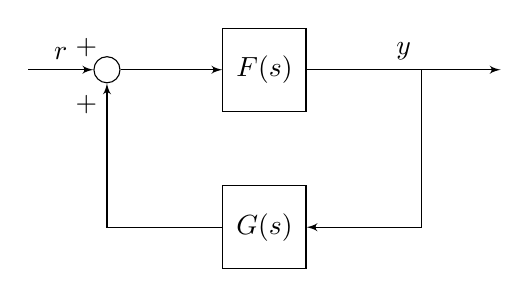
\begin{tikzpicture}[auto, node distance=2cm,>=latex']
  \node [input, name=rinput]                            (rinput)    {};
  \node [sum, right of=rinput]                          (sum)       {};
  \node [block, right of=sum]                           (blocka)    {$F(s)$};
  \node [block, below of=blocka]                        (blockb)    {$G(s)$};
  \node [tmp, below of=sum]                             (tmp1)      {};
  \node [tmp, right of=blockb]                          (tmp2)      {};
  \node [tmp, above of=tmp2]                            (tmp3)      {};
  \node [output, right of=blocka, node distance=3cm]    (output)    {};

  \draw [->] (rinput) -- node{$r$} (sum);
  \draw [->] (sum) -- (blocka);
  \draw [->] (blocka) -- node [name=y] {$y$}(output);
  \draw [->] (tmp3) -- (tmp2) -- (blockb);
  \draw [->] (blockb) -- (tmp1) -- node[pos=0.85] {$+$} node[pos=1.25] {$+$} (sum);
\end{tikzpicture}\\
%
%
Överföringsfunktionen för ett sådant system är som bekant
\begin{align*}
  \frac{y}{r} = \frac{F(s)}{1 - F(s)G(s)}
\end{align*}
%
%
Om vi tittar på den inre återkopplingen, som vi nyss markerade, och ritar om den på standardformen får vi:\\
%
%
\begin{tikzpicture}[auto, node distance=2cm,>=latex']
  \node [input, name=rinput]                            (rinput)    {};
  \node [block, right of=rinput]                        (block0)    {$0.4$};
  \node [sum, right of=block0]                          (sum)       {};
  \node [block, right of=sum]                           (blocka)    {$-\frac{1}{1+2s}$};
  \node [block, below of=blocka]                        (blockb)    {$0.5$};
  \node [tmp, below of=sum]                             (tmp1)      {};
  \node [tmp, right of=blockb]                          (tmp2)      {};
  \node [tmp, above of=tmp2]                            (tmp3)      {};
  \node [output, right of=blocka, node distance=3cm]    (output)    {};

  \draw [->] (rinput) -- node{$i$} (block0);
  \draw [->] (block0) -- (sum) -- (blocka);
  \draw [->] (blocka) -- node [name=y] {$o$}(output);
  \draw [->] (tmp3) -- (tmp2) -- (blockb);
  \draw [->] (blockb) -- (tmp1) -- node[pos=0.85] {$+$} node[pos=1.25] {$+$} (sum);
\end{tikzpicture}\\
%
%
Sätter vi upp överföringsfunktionen för delsystemet så får vi
\begin{align*}
  \frac{o}{i} = 0.4 \frac{-\frac{1}{1+2s}}{1-(-\frac{1}{1+2s})0.5}
\end{align*}
%
Vi kan förenkla systemet genom att börja med att förlänga med $1+2s$:
\begin{align*}
  \frac{o}{i} = -0.4 \frac{\frac{1}{1+2s}}{1+\frac{1}{1+2s}0.5} = -0.4 \frac{1+2s}{1+2s} \cdot \frac{\frac{1}{1+2s}}{1+\frac{1}{1+2s}0.5} =\\
  -0.4 \frac{\frac{1}{1+2s}(1+2s)}{(1+2s) + \frac{1}{1+2s}0.5(1+2s)} = -0.4 \frac{1}{(1+2s) + 0.5} = -\frac{0.4}{2s + 1.5}
\end{align*}
%
%
Vi kan nu ersätta den inre återkopplingen med en låda med den inre återkopp\-lingens överföringsfunktion:\\
%
%
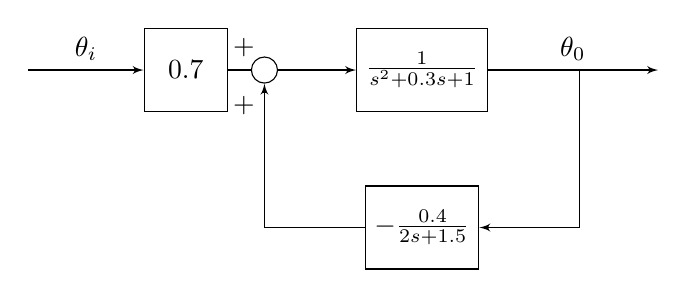
\begin{tikzpicture}[auto, node distance=2cm,>=latex']
  \node [input, name=rinput]                            (rinput)    {};
  \node [block, right of=rinput]                        (blocka)    {$0.7$};
  \node [sum, right of=blocka]                          (sum)       {};
  \node [block, right of=sum]                           (blockb)    {$\frac{1}{s^2 + 0.3s + 1}$};
  \node [block, below of=blockb]                        (blockc)    {$-\frac{0.4}{2s + 1.5}$};
  \node [tmp, below of=sum]                             (tmp1)      {};
  \node [tmp, right of=blockc]                          (tmp2)      {};
  \node [tmp, above of=tmp2]                            (tmp3)      {};
  \node [output, right of=blockb, node distance=3cm]    (output)    {};

  \draw [->] (rinput) -- node{$\theta_i$} (blocka);
  \draw [->] (blocka) -- (sum) -- (blockb);
  \draw [->] (blockb) -- node [name=y] {$\theta_0$}(output);
  \draw [->] (tmp3) -- (tmp2) -- (blockc);
  \draw [->] (blockc) -- (tmp1) -- node[pos=0.85] {$+$} node[pos=1.25] {$+$} (sum);
\end{tikzpicture}\\
%
%
På precis samma sätt som ovan kan vi nu förenkla systemet genom att sätta upp dess överföringsfunktion.
\begin{align*}
  \frac{\theta_0}{\theta_i} = 0.7 \frac{\frac{1}{s^2 + 0.3s + 1}}{1-\frac{1}{s^2 + 0.3s + 1} (-\frac{0.4}{2s+1.5})}
\end{align*}
%
Vi förlänger med $(s^2 + 0.3s + 1)(2s+1.5)$:
%
\begin{align*}
  \frac{\theta_0}{\theta_i} = 0.7 \frac{(s^2 + 0.3s + 1)(2s+1.5)}{(s^2 + 0.3s + 1)(2s+1.5)} \cdot \frac{\frac{1}{s^2 + 0.3s + 1}}{1+\frac{1}{s^2 + 0.3s + 1}\cdot \frac{0.4}{2s+1.5}} = \\
  0.7 \frac{\frac{1}{s^2 + 0.3s + 1} (s^2 + 0.3s + 1)(2s+1.5)}{(s^2 + 0.3s + 1)(2s+1.5) + \frac{1}{s^2 + 0.3s + 1}\cdot \frac{0.4}{2s+1.5} (s^2 + 0.3s + 1)(2s+1.5)} = \\
  0.7 \frac{2s+1.5}{(s^2 + 0.3s + 1)(2s+1.5) + 0.4} = 0.7 \frac{2(s+0.75)}{2((s^2 + 0.3s + 1)(s+0.75) + 0.2)} = \\
  \frac{0.7(s+0.75)}{s^3 + 1.05s^2 + 1.225s + 0.95}
\end{align*}
%
%
På blockschemaform:\\
%
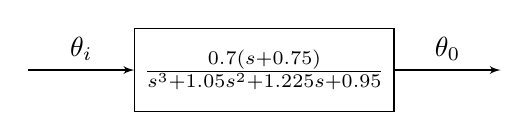
\begin{tikzpicture}[auto, node distance=2cm,>=latex']
  \node [input, name=rinput]                            (rinput)    {};
  \node [block, right of=rinput, node distance=3cm]     (blocka)    {$\frac{0.7(s+0.75)}{s^3 + 1.05s^2 + 1.225s + 0.95}$};
  \node [output, right of=blocka, node distance=3cm]    (output)    {};

  \draw [->] (rinput) -- node{$\theta_i$} (blocka);
  \draw [->] (blocka) -- node [name=y] {$\theta_0$}(output);
\end{tikzpicture}\\
%
%
Fördelen med denna lösningsmetod är att vi mekaniskt arbetar med det givna blockschemat. Nackdelen är att vi har ett positivt återkopplat system (det vill säga, signalerna till alla summeringspunkterna i systemet adderas), vilket inte används lika mycket i Reglerteknikkursen. Detta är inte ett problem, utan det är mest att vi är lite mer ovana vid att ställa upp positivt återkopplade system.
\\\\\\
%
%
%
\textbf{Alternativ 2:} Det lösningsförslag som presenteras i facit har fördelen att vi har ett negativt återkopplat system (det vill säga, signalerna till alla summeringspunkterna i systemet subtraheras), vilket vi ju räknar oftare på. Vi kan flytta boxen $-1$ fram över delningspunkten, och få följande blockdiagram:\\
%
%
\begin{tikzpicture}[auto, node distance=2cm,>=latex']
  \node [input, name=rinput]                            (rinput)    {};
  \node [block, right of=rinput]                        (block07)   {$0.7$};
  \node [sum, right of=block07]                         (suma)      {};
  \node [block, below of=suma, node distance=1.5cm]     (blockm2)   {$-1$};
  \node [tmp, below of=blockm2, node distance=1.5cm]    (tmp1)      {};
  \node [tmp, below of=tmp1, node distance=2cm]         (tmp2)      {};
  \node [block, right of=tmp1, node distance=1cm]       (blockm1)   {$-1$};
  \node [block, right of=blockm1, node distance=1.5cm]  (block05)   {$0.5$};
  \node [tmp, right of=block05, node distance=1cm]      (tmp3)      {};
  \node [block, below of=block05]                       (blocka)    {$\frac{1}{1+2s}$};
  \node [sum, right of=blocka]                          (sumb)      {};
  \node [block, right of=sumb, node distance=1.5cm]     (block04)   {$0.4$};
  \node [tmp, right of=block04, node distance=1cm]      (tmp4)      {};
  \node [block, right of=suma]                          (flygplan)  {$\frac{1}{s^2 + 0.3s + 1}$};
  \node [output, right of=flygplan, node distance=7cm]  (output)    {};

  \draw [->] (rinput) -- node{$\theta_i$} (block07);
  \draw [->] (block07) -- (suma);
  \draw [->] (suma) -- (flygplan);
  \draw [->] (flygplan) -- node [name=y] {$\theta_0$}(output);
  \draw [->] (sumb) -- (blocka);
  \draw [->] (blocka) -- (tmp2) -- (tmp1) -- (blockm2);
  \draw [->] (blockm2) -- node[pos=0.95] {$+$} node[pos=1.45] {$+$} (suma);
  \draw [->] (tmp1) -- (blockm1) -- (block05);
  \draw [->] (block05) -- (tmp3) -- node[pos=0.95] {$+$} node[pos=1.25] {$+$} (sumb);
  \draw [->] (block04) -- (sumb);
  \draw [->] (y) -- (tmp4) -- (block04);
\end{tikzpicture}\\
%
%
I den övre summeringspunkten så adderar vi en negerad signal, vilket är samma sak som att subtrahera signalen. Vi kan alltså ersätta additionstecknet med ett subtraktionstecken, och ta bort boxen med $-1$. På samma sätt gör vi i den inre återkopplingen; den återkopplande signalen kommer vara negerad, och vi kan därför ersätta additionstecknet i den undre summeringspunkten med ett subtraktionstecken:\\
%
%
\begin{tikzpicture}[auto, node distance=2cm,>=latex']
  \node [input, name=rinput]                            (rinput)    {};
  \node [block, right of=rinput]                        (block07)   {$0.7$};
  \node [sum, right of=block07, node distance=1.2cm]    (suma)      {};
  \node [tmp, below of=suma]                            (tmp1)      {};
  \node [tmp, below of=tmp1]                            (tmp2)      {};
  \node [block, right of=tmp2, node distance=1.5cm]     (blocka)    {$\frac{1}{1+2s}$};
  \node [block, above of=blocka]                        (block05)   {$0.5$};
  \node [tmp, right of=block05, node distance=1cm]      (tmp3)      {};
  \node [sum, right of=blocka]                          (sumb)      {};
  \node [block, right of=sumb, node distance=1cm]       (block04)   {$0.4$};
  \node [tmp, right of=block04, node distance=0.9cm]    (tmp4)      {};
  \node [block, above of=block05]                       (flygplan)  {$\frac{1}{s^2 + 0.3s + 1}$};
  \node [output, right of=flygplan, node distance=5cm]  (output)    {};

  \draw [->] (rinput) -- node{$\theta_i$} (block07);
  \draw [->] (block07) -- (suma);
  \draw [->] (suma) -- (flygplan);
  \draw [->] (flygplan) -- node [name=y] {$\theta_0$}(output);
  \draw [->] (sumb) -- (blocka);
  \draw [->] (blocka) -- (tmp2) -- (tmp1) -| node[pos=0.95] {$-$} node[pos=1.15] {$+$} (suma);
  \draw [->] (tmp1) -- (block05);
  \draw [->] (block05) -- (tmp3) -- node[pos=0.85] {$-$} node[pos=1.25] {$+$} (sumb);
  \draw [->] (block04) -- (sumb);
  \draw [->] (y) -- (tmp4) -- (block04);
\end{tikzpicture}\\
%
Standardformen för att rita en enkel negativ återkoppling är:\\
%
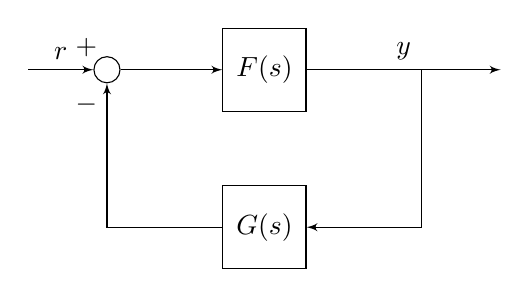
\begin{tikzpicture}[auto, node distance=2cm,>=latex']
  \node [input, name=rinput]                            (rinput)    {};
  \node [sum, right of=rinput]                          (sum)       {};
  \node [block, right of=sum]                           (blocka)    {$F(s)$};
  \node [block, below of=blocka]                        (blockb)    {$G(s)$};
  \node [tmp, below of=sum]                             (tmp1)      {};
  \node [tmp, right of=blockb]                          (tmp2)      {};
  \node [tmp, above of=tmp2]                            (tmp3)      {};
  \node [output, right of=blocka, node distance=3cm]    (output)    {};

  \draw [->] (rinput) -- node{$r$} (sum);
  \draw [->] (sum) -- (blocka);
  \draw [->] (blocka) -- node [name=y] {$y$}(output);
  \draw [->] (tmp3) -- (tmp2) -- (blockb);
  \draw [->] (blockb) -- (tmp1) -- node[pos=0.85] {$-$} node[pos=1.25] {$+$} (sum);
\end{tikzpicture}\\
%
%
Överföringsfunktionen för ett sådant system är som bekant
\begin{align*}
  \frac{y}{r} = \frac{F(s)}{1 + F(s)G(s)}
\end{align*}
%
%
Om vi tittar på den inre återkopplingen, och ritar om den på standardformen får vi:\\
%
%
\begin{tikzpicture}[auto, node distance=2cm,>=latex']
  \node [input, name=rinput]                            (rinput)    {};
  \node [block, right of=rinput]                        (block0)    {$0.4$};
  \node [sum, right of=block0]                          (sum)       {};
  \node [block, right of=sum]                           (blocka)    {$\frac{1}{1+2s}$};
  \node [block, below of=blocka]                        (blockb)    {$0.5$};
  \node [tmp, below of=sum]                             (tmp1)      {};
  \node [tmp, right of=blockb]                          (tmp2)      {};
  \node [tmp, above of=tmp2]                            (tmp3)      {};
  \node [output, right of=blocka, node distance=3cm]    (output)    {};

  \draw [->] (rinput) -- node{$i$} (block0);
  \draw [->] (block0) -- (sum) -- (blocka);
  \draw [->] (blocka) -- node [name=y] {$o$}(output);
  \draw [->] (tmp3) -- (tmp2) -- (blockb);
  \draw [->] (blockb) -- (tmp1) -- node[pos=0.85] {$-$} node[pos=1.25] {$+$} (sum);
\end{tikzpicture}\\
%
%
Sätter vi upp överföringsfunktionen för delsystemet så får vi
\begin{align*}
  \frac{o}{i} = 0.4 \frac{\frac{1}{1+2s}}{1+\frac{1}{1+2s}0.5}
\end{align*}
%
Vi kan förenkla systemet genom att börja med att förlänga med $1+2s$:
\begin{align*}
  \frac{o}{i} = 0.4 \frac{\frac{1}{1+2s}}{1+\frac{1}{1+2s}0.5} = 0.4 \frac{1+2s}{1+2s} \cdot \frac{\frac{1}{1+2s}}{1+\frac{1}{1+2s}0.5} =\\
  0.4 \frac{\frac{1}{1+2s}(1+2s)}{(1+2s) + \frac{1}{1+2s}0.5(1+2s)} = 0.4 \frac{1}{(1+2s) + 0.5} = \frac{0.4}{2s + 1.5}
\end{align*}
%
%
Vi kan nu ersätta den inre återkopplingen med en låda med den inre återkopp\-lingens överföringsfunktion:\\
%
%
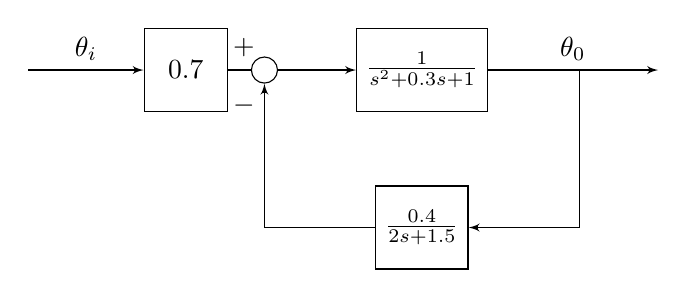
\begin{tikzpicture}[auto, node distance=2cm,>=latex']
  \node [input, name=rinput]                            (rinput)    {};
  \node [block, right of=rinput]                        (blocka)    {$0.7$};
  \node [sum, right of=blocka]                          (sum)       {};
  \node [block, right of=sum]                           (blockb)    {$\frac{1}{s^2 + 0.3s + 1}$};
  \node [block, below of=blockb]                        (blockc)    {$\frac{0.4}{2s + 1.5}$};
  \node [tmp, below of=sum]                             (tmp1)      {};
  \node [tmp, right of=blockc]                          (tmp2)      {};
  \node [tmp, above of=tmp2]                            (tmp3)      {};
  \node [output, right of=blockb, node distance=3cm]    (output)    {};

  \draw [->] (rinput) -- node{$\theta_i$} (blocka);
  \draw [->] (blocka) -- (sum) -- (blockb);
  \draw [->] (blockb) -- node [name=y] {$\theta_0$}(output);
  \draw [->] (tmp3) -- (tmp2) -- (blockc);
  \draw [->] (blockc) -- (tmp1) -- node[pos=0.85] {$-$} node[pos=1.25] {$+$} (sum);
\end{tikzpicture}\\
%
%
På precis samma sätt som ovan kan vi nu förenkla systemet genom att sätta upp dess överföringsfunktion.
\begin{align*}
  \frac{\theta_0}{\theta_i} = 0.7 \frac{\frac{1}{s^2 + 0.3s + 1}}{1+\frac{1}{s^2 + 0.3s + 1}\cdot \frac{0.4}{2s+1.5}}
\end{align*}
%
%
Vi förlänger med $(s^2 + 0.3s + 1)(2s+1.5)$:
%
\begin{align*}
  \frac{\theta_0}{\theta_i} = 0.7 \frac{(s^2 + 0.3s + 1)(2s+1.5)}{(s^2 + 0.3s + 1)(2s+1.5)} \cdot \frac{\frac{1}{s^2 + 0.3s + 1}}{1+\frac{1}{s^2 + 0.3s + 1}\cdot \frac{0.4}{2s+1.5}} = \\
  0.7 \frac{\frac{1}{s^2 + 0.3s + 1} (s^2 + 0.3s + 1)(2s+1.5)}{(s^2 + 0.3s + 1)(2s+1.5) + \frac{1}{s^2 + 0.3s + 1}\cdot \frac{0.4}{2s+1.5} (s^2 + 0.3s + 1)(2s+1.5)} = \\
  0.7 \frac{2s+1.5}{(s^2 + 0.3s + 1)(2s+1.5) + 0.4} = 0.7 \frac{2(s+0.75)}{2((s^2 + 0.3s + 1)(s+0.75) + 0.2)} = \\
  \frac{0.7(s+0.75)}{s^3 + 1.05s^2 + 1.225s + 0.95}
\end{align*}
%
%
På blockschemaform:\\
%
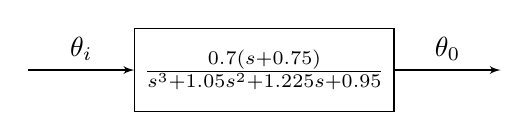
\begin{tikzpicture}[auto, node distance=2cm,>=latex']
  \node [input, name=rinput]                            (rinput)    {};
  \node [block, right of=rinput, node distance=3cm]     (blocka)    {$\frac{0.7(s+0.75)}{s^3 + 1.05s^2 + 1.225s + 0.95}$};
  \node [output, right of=blocka, node distance=3cm]    (output)    {};

  \draw [->] (rinput) -- node{$\theta_i$} (blocka);
  \draw [->] (blocka) -- node [name=y] {$\theta_0$}(output);
\end{tikzpicture}\\
%
%
Samma svar erhålls alltså oavsett angreppssätt.




\subsection{3a}
Som framgår av differentialekvationen och texten så har vi två funktioner som beror av tiden: $u(t)$ och $N(t)$. Vi har också konstanter: $J$, $R$, $K_T$, $K_G$ och $K_E$. Uppgiften är att räkna ut den konstanta spänningen $u_0$ för det konstanta varvtalet $N_0$, det vill säga ersätta de variabla funktionerna $N(t)$ och $u(t)$ med konstanterna $N_0$ respektive $u_0$, och sedan bryta ut $u_0$.

\begin{align*}
  J \frac{dN_0}{dt} + K_G{N_0}^2 = \frac{K_T}{R}(u_0 - K_EN_0)
\end{align*}
%
Den första termen, $\frac{dN_0}{dt}$, deriverar en konstant med avseende på tiden. En derivata av en konstant är noll, varpå den termen faller bort. Vi får:

\begin{align*}
  0 + K_G{N_0}^2 &= \frac{K_T}{R}u_0 - \frac{K_T}{R}K_EN_0\\
  u_0 &= \frac{K_G{N_0}^2R}{K_T} + K_EN_0
\end{align*}
%


\subsection{3b}
Se sektion \ref{sec:linjärisering} för bakgrund till linjärisering. Vi börjar med att kalla differentialekvationen för $g$ och flyttar över alla termer till samma sida.

\begin{align*}
  g(u, N) = \underbrace{J \frac{dN(t)}{dt}}_{\text{Term 1}} + \underbrace{K_G{N(t)}^2\frac{ }{ }}_{\text{Term 2}} + \underbrace{\frac{K_T K_E}{R} N(t)}_{\text{Term 3}} - \underbrace{\frac{K_T}{R}u(t)}_{\text{Term 4}}
\end{align*}
Linjärisera!
\begin{align*}
  g(u, N) \approx \left. \frac{\partial g}{\partial u}\right|_{u_0, N_0}(u - u_0) + \left. \frac{\partial g}{\partial N}\right|_{u_0, N_0}(N - N_0)
\end{align*}

%Vi ska alltså summera den partiella deriveran av $g$ med avseende på $u$ med den partiella derivatan av $g$ med avseende på $N$.
När vi först partialderiverar med avseende på $u$ kommer alla termer som inte innehåller $u$ (Term 1, Term 2 och Term 3) betraktas som konstanter. Derivatan av en konstant är som bekant noll, vilket gör att alla termer ej innehållande $u$ då försvinner.

\begin{align*}
  \frac{\partial g}{\partial u} = -\frac{K_T}{R}
\end{align*}

På samma sätt gäller att när vi partialderiverar med avseende på $N$, så kommer Term 4 som inte innehåller $N$ att bli 0. Vi får:

\begin{align*}
  \frac{\partial g}{\partial N} = J\frac{d}{dt} + 2K_G N + \frac{K_T K_E}{R}
\end{align*}

Term 1 innehåller en derivering av $N(t)$ med avseende på $t$, men när vi nu partialderiverar $g$, så gör vi det med avseende på $N$. Tidsderiveringen blir alltså kvar, men inte funktionen $N$.

Vi linjäriserar enligt uppgiften i arbetspunkten $(u_0, N_0)$, vilket innebär att vi stoppar in värdet $u_0$ i funktionen $u$ och stoppar in $N_0$ i funktionen $N$. Med lite slappt språkbruk kan vi säga att vi ``ersätter'' $u$ med $u_0$ och $N$ med $N_0$. Det är detta som avses med beteckningarna $\left. \frac{\partial g}{\partial u} \right|_{u_0, N_0}$ respektive $\left. \frac{\partial g}{\partial N} \right|_{u_0, N_0}$.

I $\frac{\partial g}{\partial N}$ ersätter vi alltså $N$ med $N_0$. Något $u$ finns inte i varken $\frac{\partial g}{\partial u}$ eller $\frac{\partial g}{\partial N}$, och något $N$ finns inte i $\frac{\partial g}{\partial u}$. För exempel på när vi har kvar termer att ersätta, se det första exemplet i Matematikrepetitionshäftet kaptiel 5.1.

\begin{align*}
  g(u, N) \approx \left. \frac{\partial g}{\partial u}\right|_{u_0, N_0}(u - u_0) + \left. \frac{\partial g}{\partial N}\right|_{u_0, N_0}(N - N_0) = \\
  -\frac{K_T}{R}(u - u_0) + \left(J\frac{d}{dt} + 2K_G N_0 + \frac{K_T K_E}{R} \right)(N - N_0)
\end{align*}

Vi sätter $\Delta N = N - N_0$ och $\Delta u = u - u_0$:

\begin{align*}
  \frac{-K_T}{R}\Delta u(t) &+ J\frac{d\Delta N(t)}{dt} + 2K_G N_0\Delta N(t) + \frac{K_T K_E}{R} \Delta N(t) = 0 \Longleftrightarrow\\
  \frac{K_T}{R}\Delta u(t) &= J\frac{d\Delta N(t)}{dt} + \left(2K_G N_0 + \frac{K_T K_E}{R} \right) \Delta N(t)
\end{align*}


\subsection{3c}
\oklarhet{Vad gör vi här egentligen?}

\begin{align*}
  \frac{\Delta N(s)}{\Delta u(s)} = \frac{\frac{K_T}{R}}{Js + 2K_G N_0 + \frac{K_T K_E}{R}} = \frac{K_T}{RJs + 2 K_G N_0 R + K_T K_E}
\end{align*}

\oklarhet{Vartifrån kommer den formen?}

Vi vill ha uttrycket på formen $\frac{K}{1 + sT}$. Tidskonstanten som det frågas efter är $T$. Det gäller för oss att algebraiskt arbeta om uttrycket så att vi får det på önskad form.

\begin{align*}
  \frac{K_T}{RJs + 2 K_G N_0 R + K_T K_E} = \frac{\frac{1}{2 K_G N_0 R + K_T K_E}}{\frac{1}{2 K_G N_0 R + K_T K_E}}\frac{K_T}{RJs + 2 K_G N_0 R + K_T K_E} = \\
  \frac{\frac{K_T}{2K_G N_0 R + K_T K_E}}{\frac{RJ}{2K_G N_0 R + K_T K_E}s + 1} = \frac{K}{Ts + 1}
\end{align*}

Vi kan nu avläsa $T$.

\begin{align*}
  T = \frac{RJ}{2K_G N_0 R + K_T K_E} = \frac{J}{2K_G N_0 + \frac{K_T K_E}{R}}
\end{align*}

Varvtalet, $N_0$, står i nämnaren, det vill säga $T$ minskar med ökat varvtal.


\subsection{4a}
Teorin bakom detta står på \bl{sid 424}.\\\\
%
I det allmänna fallet så gäller
\begin{align*}
  \dot{x}(t) =~& Ax(t) + Bu(t) \\
  y(t) =~& Cx(t) + Du(t)
\end{align*}
och i vårt fall så har vi
\begin{align*}
  \dot{x}(t) =& \begin{bmatrix}0 & 1 \\ 0 & 0\end{bmatrix} x(t) + \begin{bmatrix}-1 \\ 1\end{bmatrix} u(t) \\
  y(t) =& \begin{bmatrix}1 & 0\end{bmatrix} x(t)\\\\
  u(t) =& -Lx(t) + K_r r(t)
\end{align*}
%
%
Då det skall finnas relativ dämpning och naturlig egenfrekvens så ska vi använda följande ekvation från det till tesen bifogade formelbladet.

\begin{align*}
  G(s) = \frac{\omega_n ^2}{s^2 + 2\zeta \omega_n s + \omega_n^2}
\end{align*}

Det karakteristiska polynomet för det slutna systemet är alltså för $\zeta = \frac{1}{\sqrt{2}}$ och $\omega_n = \sqrt{2}$:

\begin{align*}
  \alpha_c(s) = s^2 + 2\zeta \omega_n s + \omega_n^2 = s^2 + 2\frac{1}{\sqrt{2}} \sqrt{2} s + (\sqrt{2})^2 = s^2 + 2s + 2
\end{align*}

Enligt (11.15) på \bl{sid 425} så gäller följande för det slutna systemet:

\begin{align*}
  \alpha_c(s) = \det(sI - A + BL)
\end{align*}

\begin{align*}
  sI - A + BL = \begin{bmatrix}s & 0 \\ 0 & s\end{bmatrix} - \begin{bmatrix}0 & 1 \\ 0 & 0\end{bmatrix} + \begin{bmatrix}-1 \\ 1\end{bmatrix}\begin{bmatrix}l_1 & l_2\end{bmatrix} = \\
  \begin{bmatrix}s & -1 \\ 0 & s\end{bmatrix} + \begin{bmatrix}-l_1 & -l_2 \\ l_1 & l_2\end{bmatrix} = \begin{bmatrix}s - l_1 & -1 -l_2 \\ l_1 & s + l_2\end{bmatrix}
\end{align*}

Hur man räknar ut determinanter står på \mhb{sid 93}.

\begin{align*}
  \det(sI - A + BL) = \det \left( \begin{bmatrix}s - l_1 & -1 -l_2 \\ l_1 & s + l_2\end{bmatrix} \right) = \\
  (s - l_1)(s + l_2) - l_1(-1 -l_2) = s^2 + (-l_1 + l_2)s + l_1
\end{align*}

Detta är alltså lika med det karakteristiska polynomet ($\alpha_c(s)$), varifrån vi kan identifiera värden på $l_1$ och $l_2$:
%
\begin{eqnarray*}
  s^2 + &(-l_1 + l_2)s &+ l_1 = \\
  s^2 + &2s &+ 2\\
\end{eqnarray*}
\vspace{-10mm}
\begin{align*}
  \left\{ \begin{array}{ll}
  -l_1 + l_2 = 2\\
  l_1 = 2
  \end{array} \right. \Longleftrightarrow
  \left\{ \begin{array}{ll}
  l_1 = 2\\
  l_2 = 4
  \end{array} \right.
\end{align*}



\subsection{4b}
Enligt (11.16) på \bl{sid 426} så gäller:

\begin{align*}
  G_{ry}(s) = C(sI - A + BL)^{-1}BK_r
\end{align*}

Vi ska alltså lösa ut $K_r$, och för att göra det behöver vi utföra lite matrismultiplikation och räkna ut inversen av $sI - A + BL$. Hur man räknar ut matrisinverser står på \mhb{sid 94}.

\begin{align*}
  G_{ry}(s) = C(sI - A + BL)^{-1}BK_r = \begin{bmatrix}1 & 0\end{bmatrix} \left(\begin{bmatrix}s - l_1 & -1 -l_2 \\ l_1 & s + l_2\end{bmatrix} \right)^{-1} \begin{bmatrix}-1 \\ 1\end{bmatrix} K_r = \\
  \begin{bmatrix}1 & 0\end{bmatrix} \left(\frac{1}{(s-l_1)(s+l_2) - l_1(-1-l_2)}\begin{bmatrix}s + l_2 & 1 +l_2 \\ -l_1 & s - l_1\end{bmatrix} \right) \begin{bmatrix}-1 \\ 1\end{bmatrix} K_r = \\
  \begin{bmatrix}1 & 0\end{bmatrix} \begin{bmatrix}s + l_2 & 1 +l_2 \\ -l_1 & s - l_1\end{bmatrix} \begin{bmatrix}-1 \\ 1\end{bmatrix} \frac{K_r}{(s-l_1)(s+l_2) - l_1(-1-l_2)} = \\
  \begin{bmatrix}1 & 0\end{bmatrix} \begin{bmatrix}-(s + l_2) + (1 +l_2) \\ l_1 + (s - l_1)\end{bmatrix} \frac{K_r}{s^2 + (-l_1 + l_2)s + l_1} = \\
  \begin{bmatrix}1 & 0\end{bmatrix} \begin{bmatrix}1 - s \\ s\end{bmatrix} \frac{K_r}{s^2 + (-l_1 + l_2)s + l_1} = \\
  (1 - s) \frac{K_r}{s^2 + (-l_1 + l_2)s + l_1} = \\
  \frac{K_r(1 - s)}{s^2 + (-l_1 + l_2)s + l_1}
\end{align*}

Sätter vi in värdena på $l_1$ och $l_2$ från a)-uppgiften så får vi:

\begin{align*}
  G_{ry}(s) = \frac{K_r(1 - s)}{s^2 + (-l_1 + l_2)s + l_1} = \frac{K_r(1 - s)}{s^2 + (-2 + 4)s + 2} = \frac{K_r(1 - s)}{s^2 + 2s + 2}
\end{align*}

Villkoret i stationaritet uppfylls genom att sätta $G_{ry}(0) = 1$:
\begin{align*}
  G_{ry}(0) = \frac{K_r(1 - 0)}{0^2 + 2\cdot 0 + 2} = \frac{K_r}{2} = 1 \Longleftrightarrow\\
  K_r = 2
\end{align*}


\section{Tenta 2013-08-22}
\subsection{1a}
Notera att uppgiften säger att $u$ är insignal, det är alltså inte ett steg som står inskrivet i differentialekvationen. Insignalen är en sinussignal, vilket innebär att vi väljer att ansätta problemet enligt nedan.
%
Laplacea med hjälp av \mhb{L8} ($\ddot{y}(t)$), \mhb{L7} ($\dot{y}(t)$), \mhb{L6} ($y(t)$) och \mhb{L4} ($u(t - 2)$):
\begin{align*}
  \ddot y(t) + 3 \dot y(t) + 2y(t) &= 3u(t-2)\\
  s^2Y(s) + 3sY(s) + 2Y(s) &= 3e^{-2s}U(s)\\
  Y(s)(s^2 + 3s + 2) &= 3e^{-2s}U(s)\\
  G(s) = \frac{Y(s)}{U(s)} = \frac{3e^{-2s}}{s^2 + 3s + 2} &= \frac{3e^{-2s}}{(s + 1)(s + 2)}
\end{align*}
%
%
Vi ersätter $s$ med $i\omega$ (det vill säga går över från s-domänen till Frekvensdomänen).
%
%
\begin{align*}
  G(i\omega) = \frac{3e^{-2i\omega}}{(i\omega + 1)(i\omega + 2)}
\end{align*}
%
%
På \mhb{sid 339} regel 7 under `Continuous Systems' ser vi att med en insignal som är $\sin(\omega t)$, så blir utsignalen $|G(i\omega)| \sin(\omega t + \arg\{ G(i\omega) \})$.

Vi börjar med att räkna ut $|G(i\omega)|$, och hur vi gör det står beskrivet på \mhb{sid 61}: $|z| = \sqrt{(\text{Re\{z\}})^2 + (\text{Im\{z\}})^2}$. På \mhb{sid 61} finns några användbara räkneregler för absolutbelopp: $|z_1 z_2| = |z_1|\cdot |z_2|$ och $\left|\frac{z_1}{z_2}\right| = \frac{|z_1|}{|z_2|}$. Vi ser också på \mhb{sid 62} att $|e^{i\theta}| = 1$.
\begin{align*}
  |G(i\omega)| = \left|\frac{3e^{-2i\omega}}{(i\omega + 1)(i\omega + 2)}\right| = \\
  \frac{|3|\cdot|e^{-2i\omega}|}{|(i\omega + 1)|\cdot|(i\omega + 2)|} = \\
  \frac{3}{\sqrt{\omega^2 + 1^2}\sqrt{\omega^2 + 2^2}}
\end{align*}

Vi räknar nu ut $\arg\{ G(i\omega) \}$, och hur vi gör det står beskrivet på \mhb{sid 62}: $\arg\{z\} = \arctan{\frac{\text{Im\{z\}}}{\text{Re\{z\}}}}$. På \mhb{sid 62} finns några användbara räkneregler för argument: $\arg\{ z_1 z_2 \} = \arg \{z_1\} + \arg \{z_2\}$ och $\arg\{ \frac{z_1}{z_2} \} = \arg\{ z_1 \} - \arg\{ z_2 \}$. Vi ser också på \mhb{sid 62} att $\arg \{e^{i\theta}\} = \theta$.

\begin{align*}
  \arg\{ G(i\omega) \} = \arg \left\{ \frac{3e^{-2i\omega}}{(i\omega + 1)(i\omega + 2)} \right\} = \\
  \arg\{ 3e^{-2i\omega} \} - \arg\{ (i\omega + 1)(i\omega + 2) \} = \\
  \arg\{ 3 \} + \arg\{ e^{-2i\omega} \} - (\arg\{ i\omega + 1\} + \arg\{ i\omega + 2 \}) = \\
  \arctan \frac{0}{3} -2\omega -(\arctan\frac{\omega}{1} + \arctan\frac{\omega}{2}) = \\
  -2\omega -\arctan\omega - \arctan\frac{\omega}{2}
\end{align*}

Vi kan nu skriva upp det hela på önskad form:

\begin{align*}
  y(t) = |G(i\omega)| \sin(\omega t + \arg\{ G(i\omega) \}) = \\
  \frac{3}{\sqrt{\omega^2 + 1}\sqrt{\omega^2 + 4}} \sin(\omega t - 2\omega -\arctan\omega - \arctan\frac{\omega}{2})
\end{align*}

\oklarhet{Varför gäller detta enbart när det är strikt stabilt? Nämn det som nödvändigt kriterium!}
\oklarhet{Kommentera begreppet ``stora $t$''.}


\section{Tenta 2013-04-05}
\subsection{5a}

Vår uppgift är att vi blivit givna $G(s)$ (vars egenskaper vi inte kan påverka), och vi ska dimensionera en regulator $F(s)$ som ändrar systemets egenskaper så att de uppfyller uppgiftens krav.

\begin{tikzpicture}[auto, node distance=2cm,>=latex']
  \node [input, name=rinput]        (rinput)    {};
  \node [sum, right of=rinput]      (sum)       {};
  \node [block, right of=sum]       (blocka)    {$F(s)$};
  \node [block, right of=blocka]    (blockb)    {$G(s)$};
  \node [tmp, below of=sum]         (tmp1)      {};
  \node [tmp, right of=blockb]      (tmp2)      {};
  \node [tmp, below of=tmp2]        (tmp3)      {};
  \node [output, right of=tmp2]     (output)    {};

  \draw [->] (rinput) -- node{$r$} (sum);
  \draw [->] (sum) -- (blocka);
  \draw [->] (blocka) -- (blockb);
  \draw [->] (blockb) -- node [name=y] {$y$}(output);
  \draw [->] (tmp2) -- (tmp3) -- (tmp1) -- node[pos=0.85] {$-$} node[pos=1.25] {$+$} (sum);
\end{tikzpicture}\\

\begin{align*}
  G(s) = \frac{e^{-s}}{s(s+1)}
\end{align*}

Från (6.30) på \bl{sid 249} ser vi att följande gäller:\\
\oklarhet{Förtydliga vad vi gör här.}
\begin{align*}
  \varphi_m - 180^\circ = \arg\{G(j\omega_c)\}
\end{align*}

På \mhb{sid 62} finns några användbara räkneregler för argument: $\arg\{ z_1 z_2 \} = \arg \{z_1\} + \arg \{z_2\}$ och $\arg\{ \frac{z_1}{z_2} \} = \arg\{ z_1 \} - \arg\{ z_2 \}$.

Överkorsningsfrekvensen ska vara $\omega_c \geq 1$ rad/s. Om vi ansätter problemet med $\omega_c = 1$:

\begin{align*}
  \arg\{G(j\cdot 1)\} = \arg\{e^{-j\cdot 1}\} - (\arg\{j\cdot 1\} + \arg\{j\cdot 1 + 1\})
\end{align*}

På \mhb{sid 62} ser vi att $\arg\{e^{i\theta}\} = \theta$. Hur vi räknar ut $\arg\{ G(i\omega) \}$ framgår av \mhb{sid 62}: $\arg\{z\} = \arctan{\frac{\text{Im\{z\}}}{\text{Re\{z\}}}}$.

\begin{align*}
  \arg\{G(j\cdot 1)\} = \arg\{e^{-j\cdot 1}\} - (\arg\{j\cdot 1\} + \arg\{j\cdot 1 + 1\}) = \\
  -1 - \arctan\frac{1}{0} - \arctan\frac{1}{1} = -1 -\arctan ( \infty ) - \arctan 1 = -1 -\frac{\pi}{2} -\frac{\pi}{4} \text{rad}
\end{align*}

Värdena på arctan kommer från tabellen på \mhb{sid 130}. På \mhb{sid 125} ser vi hur vi konverterar mellan grader och radianer.

\begin{align*}
  \arg\{G(j\cdot 1)\} = -1 -\frac{\pi}{2} -\frac{\pi}{4} \text{rad} = (-1 -\frac{\pi}{2} -\frac{\pi}{4})\frac{180}{\pi}^\circ \approx -192.3^\circ
\end{align*}

Fasmarginalen som systemet redan har:
\begin{align*}
  \Phi_m - 180^\circ = \arg\{G(j\omega_c)\} \approx 192.3^\circ\\
  \Phi_m \approx 180^\circ - 192.3^\circ = -12.3^\circ
\end{align*}

Alltså, den fasmarginal som $G$ har är $-12.3^\circ$. Vill vill dimensionera $F$ så att $FG \geq 30^\circ$.

\begin{align*}
  \varphi_{m_{\text{ny}}} = 30^\circ - \Phi_m \approx 42.3^\circ
\end{align*}

Vi ska alltså höja fasmarginalen med $42.3^\circ$. Att höja fasmarginalen innebär att vi ska använda en PD-regulator.


\subsection{5b}
Från formelbladet bifogat tesen så ser vi att en PD-regulator har följande ekvation:

\begin{align*}
  F_{PD}(s) = K_p \frac{1+s\tau_d}{1+\frac{s\tau_d}{b}}
\end{align*}

Att dimensionera en regulator, vilket uppgiften ber oss göra, innebär i vårt fall att bestämma värdena i formeln, det vill säga hitta värdena på $K_p$, $\tau_d$ och $b$. Från formelbladet bifogat tesen ser vi också att följande gäller:

\begin{align*}
  b = \frac{1 + \sin \varphi_{max}}{1 - \sin \varphi_{max}}\\
  \omega_{\varphi_{max}} = \sqrt{b}/T
\end{align*}

Vi har att $\varphi_{max} = 42.3^\circ$ och $\omega_{\varphi_{max}} = 1$. Av någon anledning så byter man beteckning mellan formlerna, så $\tau_d = T$.\\
\oklarhet{Varför är $T = \tau_d$?}

\begin{align*}
  b = \frac{1 + \sin \varphi_{max}}{1 - \sin \varphi_{max}} = \frac{1 + \sin 42.3}{1 - \sin 42.3} \approx 5\\
  \omega_{\varphi_{max}} = \sqrt{b}/T \Longleftrightarrow 1 = \sqrt{5}/T \Longleftrightarrow T = \sqrt{5}
\end{align*}

Vi har nu bestämt $b$ och $T = \tau_d$, och kvar står att bestämma $K_p$. Följande samband gäller tydligen alltid\\
\oklarhet{Referens?}

\begin{align*}
  |L(i\omega)| = 1
\end{align*}

Som bekant är $L(i\omega) = G(i\omega)F(i\omega)$. Vi kan därmed ställa upp följande:

\begin{align*}
  1 = |L(i\omega)| = |G(i\omega)F(i\omega)|
\end{align*}

Vi vill med andra ord räkna ut absolutbeloppet av $|G(j\omega_{\varphi_{max}})F(j\omega_{\varphi_{max}})| = |G(j\cdot1)F(j\cdot1)| = |G(j)F(j)|$, och hur vi gör det står beskrivet på \mhb{sid 61}: $|z| = \sqrt{(\text{Re\{z\}})^2 + (\text{Im\{z\}})^2}$. På \mhb{sid 61} finns några användbara räkneregler för absolutbelopp: $|z_1 z_2| = |z_1|\cdot |z_2|$ och $\left|\frac{z_1}{z_2}\right| = \frac{|z_1|}{|z_2|}$. Vi ser också på \mhb{sid 62} att $|e^{i\theta}| = 1$.


\begin{align*}
  1 = |L(i)| = |G(i)F(i)| = |G(i)|\cdot|F(i)| = \left | \frac{e^{-j}}{j(j+1)} \right | \left | K_p\frac{1+j\sqrt{5}}{1 + \frac{j \sqrt{5}}{5}} \right | = \\
  \left | \frac{e^{-j}}{-1+j} \right | \left | K_p\frac{1+j\sqrt{5}}{1 + \frac{j}{\sqrt{5}}} \right | =
  \left | \frac{e^{-j}}{-1+j} \right | \left | K_p\frac{\sqrt{5}+5j}{\sqrt{5} + j} \right | =
  \frac{|e^{-j}|}{|-1+j|} \cdot |K_p| \frac{|\sqrt{5}+5j|}{|\sqrt{5} + j|} = \\
  \frac{1}{\sqrt{(-1)^2 + 1^2}} \cdot |K_p| \frac{\sqrt{(\sqrt{5})^2 + 5^2}}{\sqrt{(\sqrt{5})^2 + 1^2}} =
  \frac{1}{\sqrt{2}} \cdot |K_p| \frac{\sqrt{30}}{\sqrt{6}} =
  |K_p| \frac{1}{\sqrt{2}} \sqrt{\frac{30}{6}} = \\
  |K_p| \frac{1}{\sqrt{2}} \sqrt{5} =
  |K_p| \frac{\sqrt{5}}{\sqrt{2}}
\end{align*}

Då $|L(i)| = 1$ så kan vi lösa ut $K_p$:

\begin{align*}
  1 = |K_p| \frac{\sqrt{5}}{\sqrt{2}} \Longleftrightarrow K_p = \frac{\sqrt{2}}{\sqrt{5}}
\end{align*}

Stoppar vi in våra värden så får vi alltså följande PD-regulator:

\begin{align*}
  F_{PD}(s) = K_p \frac{1+s\tau_d}{1+\frac{S\tau_d}{b}} = \frac{\sqrt{2}}{\sqrt{5}} \cdot \frac{1+\sqrt{5}s}{1+\frac{\sqrt{5}s}{5}} =
  \frac{\sqrt{2}}{\sqrt{5}} \cdot \frac{1+\sqrt{5}s}{1+\frac{s}{\sqrt{5}}} = \frac{\sqrt{2}+\sqrt{10}s}{\sqrt{5} + s}
\end{align*}




%\section{Apa bepa}
%\begin{tikzpicture}[
%    scale=1.5,
%    axis/.style={very thick, ->, >=stealth'},
%    important line/.style={thick},
%    dashed line/.style={dashed, thin},
%    pile/.style={thick, ->, >=stealth', shorten <=2pt, shorten
%    >=2pt},
%    every node/.style={color=black}
%    ]
%    % Draw axes
%    \draw[axis] (-3,0) -- (0.5,0) node (xaxis) [right] {$x$};
%    \draw[axis] (0,-2) -- (0,2) node (yaxis) [above] {$y$};
%%    \draw [<->,thick] (0,2) node (yaxis) [above] {$y$}
%%        |- (3,0) node (xaxis) [right] {$x$};
%    % Draw two intersecting lines
%    \draw (0,0) coordinate (a_1) -- (2,1.8) coordinate (a_2);
%    \draw (0,0) coordinate (a_1) -- (-2,1) coordinate (a_3);
%    \draw (0,0) coordinate (a_1) -- (-2,-1) coordinate (a_4);
%    \draw (0,1.5) coordinate (b_1) -- (2.5,0) coordinate (b_2);
%    % Calculate the intersection of the lines a_1 -- a_2 and b_1 -- b_2
%    % and store the coordinate in c.
%    \coordinate (c) at (intersection of a_1--a_2 and b_1--b_2);
%    % Draw lines indicating intersection with y and x axis. Here we use
%    % the perpendicular coordinate system
%    \draw[dashed] (yaxis |- c) node[left] {$y'$}
%        -| (xaxis -| c) node[below] {$x'$};
%\end{tikzpicture}


\section{Blockdiagram}
Introduktionsvideo på enkel nivå:\\
\href{http://www.youtube.com/watch?v=Wj_vfeuksUM}{http://www.youtube.com/watch?v=Wj\_vfeuksUM}

Exempel på blockdiagramsreduktion:\\
\href{http://www.youtube.com/watch?v=rNlshpOoyxU}{http://www.youtube.com/watch?v=rNlshpOoyxU}

Exempel på blockdiagramsreduktion:\\
\href{http://www.youtube.com/watch?v=5_DpDB4CWEE}{http://www.youtube.com/watch?v=5\_DpDB4CWEE}

Föreläsning om blockdiagram:\\
\href{https://www.youtube.com/watch?v=X4hPVxZlrPU&list=PL5105727DD6E8DE98&index=6}{https://www.youtube.com/watch?v=X4hPVxZlrPU\\\&list=PL5105727DD6E8DE98\&index=6}


\section{State Space}
Introduktionsvideo som förklarar lite varför det är gött och lite om hur det fungerar:\\
\href{https://www.youtube.com/watch?v=-k2a5d-X1Gc}{https://www.youtube.com/watch?v=-k2a5d-X1Gc}


\section{Frekvenssvar och Bodediagram}
Föreläsning i rätt snabbt tempo om frekvenssvar och bodediagram:\\
\href{https://www.youtube.com/watch?v=PVV0f6KfjNg&index=6&list=PL5105727DD6E8DE98}{https://www.youtube.com/watch?v=PVV0f6KfjNg\\\&index=6\&list=PL5105727DD6E8DE98}

Samma föreläsning fast i långsammare tempo:\\
\href{https://www.youtube.com/watch?v=VfmV0vkc-ks&index=7&list=PL5105727DD6E8DE98}{https://www.youtube.com/watch?v=VfmV0vkc-ks\\\&index=7\&list=PL5105727DD6E8DE98}

Frekvenssvar och stabilitet:\\
\href{https://www.youtube.com/watch?v=-YLavh8mIVk&index=8&list=PL5105727DD6E8DE98}{https://www.youtube.com/watch?v=-YLavh8mIVk\\\&index=8\&list=PL5105727DD6E8DE98}


\section{Linjärisering}
\label{sec:linjärisering}
Att linjärisera betyder att vi gör en linjär approximering av en funktion på en viss punkt. Om vi till exempel har ett krångligt system, så kan vi förenkla arbetet genom att lägga en tangent på en punkt vi är extra intresserade av, och räkna på tangenten istället, då tangenten är lik systemet i just den punkten.

Linjäriseringsuppgifter är ju kul att få på tentan, särskilt när det kommer till flervariabelsuppgifter, vilket kanske 5\% av datastudenter behärskar. Fördelen med den här typen av uppgifter är att de är rätt lätta poäng. Hur man räknar står beskrivet i Matematikrepetitionshäftet från kursen, se kapitel 5.


\section{Partialbråksuppdelning}
\label{sec:partialbråksuppdelning}
Partialbråksuppdelning är kanske inte något man jobbar med varje dag, så det är rostigt för många. Det är dock ganska lätt. Partialbråksuppdelning används flitigt både i kurserna Reglerteknik och Transformer, Signaler och System, så om det sitter löst så är det bara att bita i det sura äpplet och lära sig. Nedan följer en lite utvidgad förklaring från Matematikrepetionshäftet kaptiel 3.

Vi antar att vi har en rationell funktion (det vill säga en kvot av två polynom) $\frac{B(s)}{A(s)}$ där $B(s)$ har lägre gradtal än $A(s)$ och där nämnaren $A(s)$ är faktoriserad så långt som det går i reella faktorer enligt tabellen nedan.

\begin{tabular}{l | l}
  Faktor i nämnaren ($A(s)$) & Ger upphov till partialbråk \\
  \hline
  $s - \alpha$       & $\frac{A_1}{s - \alpha}$ \\
  $(s - \alpha)^n$   & $\frac{A_1}{s - \alpha} + \frac{A_2}{(s - \alpha)^2} + ... + \frac{A_n}{(s - \alpha)^n}$ \\
  $s^2 + as + b$     & $\frac{B_1s + C_1}{s^2 + as + b}$ \\
  $(s^2 + as + b)^n$ & $\frac{B_1s + C_1}{s^2 + as + b} + \frac{B_2s + C_2}{(s^2 + as + b)^2} + ... + \frac{B_ns + C_n}{(s^2 + as + b)^n}$
\end{tabular}

I \mhb{sid 120} står detta kort nämnt, så man behöver inte memorera det utantill. Sätter man samtliga partialbråk på gemensam nämnare så får man ett ekvationssystem med entydig lösning. Exempel:

\begin{align}
  \frac{2s^2 + s -3}{(s+1)^2(s+2)} &= \frac{A_1}{s+1} + \frac{A_2}{(s+1)^2} + \frac{A_3}{s+2} \label{eqn:partfracA}\\
  (s+1)^2(s+2) \frac{2s^2 + s -3}{(s+1)^2(s+2)} &= (s+1)^2(s+2) \left( \frac{A_1}{s+1} + \frac{A_2}{(s+1)^2} + \frac{A_3}{s+2} \right) \label{eqn:partfracB}
\end{align}
\vspace{-7mm}
\begin{align}
  %2s^2 + s -3 &= \frac{A_1}{s+1}(s+1)^2(s+2) + \frac{A_2}{(s+1)^2}(s+1)^2(s+2) + \frac{A_3}{s+2}(s+1)^2(s+2) &\Longleftrightarrow \\
  2s^2 + s -3 &= A_1(s+1)(s+2) + A_2(s+2) + A_3(s+1)^2 \label{eqn:partfracC}\\
  2s^2 + s -3 &= s^2A_1 + 3sA_1 + 2A_1 + A_2s + 2A_2 + A_3s^2 + 2sA_3 + A_3 \label{eqn:partfracD}\\
  2s^2 + s -3 &= (A_1 + A_3)s^2 + (3A_1 + A_2 + 2A_3)s + (2A_1 + 2A_2 + A_3) \label{eqn:partfracE}
\end{align}

Vi utgår från problemet i vänsterledet i (\ref{eqn:partfracA}), och partialbråksuppdelar det enligt tabellen, varpå högerledet i (\ref{eqn:partfracA}) erhålls. I steg (\ref{eqn:partfracB}) så multiplicerar vi båda sidor av ekvationen med nämnaren i vänsterledet i (\ref{eqn:partfracA}). Vi förenklar det hela i steg (\ref{eqn:partfracC}) och (\ref{eqn:partfracD}). I (\ref{eqn:partfracE}) så ``klumpar vi ihop'' alla koefficienter till de olika gradtalen av $s$. Vi kan nu identifiera koefficienterna:

\begin{align*}
  s^2 &: A_1 + A_3 = 2\\
  s^1 &: 3A_1 + A_2 + 2A_3 = 1\\
  s^0 &: 2A_1 + 2A_2 + A_3 = -3
\end{align*}

Uttryckt lite slarvigt, om vi betraktar (\ref{eqn:partfracE}) så ser vi att koefficienterna till $s^2$ är $A_1 + A_3$ i högerledet, och detta är lika med $2$ i vänsterledet. Koefficienterna till $s^1 = s$ är $3A_1 + A_2 + 2A_3$ i högerledet och $1$ i vänsterledet. Koefficenterna till $s^0 = 1$ är $2A_1 + 2A_2 + A_3$ i högerledet och $-3$ i vänsterledet. Vi har nu tre ekvationer och tre obekanta variabler som vi vill lösa ut. Detta kan man göra på lite olika sätt. Jag löser det med matriser, men tycker du att det verkar krångligt så använd för all del ditt sätt att lösa det. Ett kort exempel på matrisalgebra finns på \mhb{sid 92}.

\begin{align*}
  \begin{amat}[r]{3}
    1  &0  &1  &2  \\
    3  &1  &2  &1  \\
    2  &2  &1  &-3
  \end{amat}
  \grstep{-3\rho_1 +\rho_2}
  &\begin{amat}[r]{3}
    1  &0  &1  &2  \\
    0  &1  &-1 &-5 \\
    2  &2  &1  &-3
  \end{amat}
  \grstep{-2\rho_1 +\rho_3}\\
  \begin{amat}[r]{3}
    1  &0  &1  &2  \\
    0  &1  &-1 &-5 \\
    0  &2  &-1 &-7
  \end{amat}
  \grstep{-2\rho_2 +\rho_3}
  &\begin{amat}[r]{3}
    1  &0  &1  &2  \\
    0  &1  &-1 &-5 \\
    0  &0  &1  &3
  \end{amat}
  \grstep{\rho_3 +\rho_2}\\
  \begin{amat}[r]{3}
    1  &0  &1  &2  \\
    0  &1  &0  &-2 \\
    0  &0  &1  &3
  \end{amat}
  \grstep{~-\rho_3 +\rho_1}
  &\begin{amat}[r]{3}
    1  &0  &0  &-1 \\
    0  &1  &0  &-2 \\
    0  &0  &1  &3
  \end{amat}
\end{align*}

Vi får alltså:
\begin{align*}
  \begin{cases}
    A_1 = -1 \\
    A_2 = -2 \\
    A_3 = 3
  \end{cases}
\end{align*}

Sätter vi in de här värdena i (\ref{eqn:partfracA}) så får vi:

\begin{align*}
  \frac{2s^2 + s -3}{(s+1)^2(s+2)} &= \frac{A_1}{s+1} + \frac{A_2}{(s+1)^2} + \frac{A_3}{s+2} =\\
  \frac{-1}{s+1} + \frac{-2}{(s+1)^2} + \frac{3}{s+2} &= -\frac{1}{s+1} -2\frac{1}{(s+1)^2} + 3\frac{1}{s+2}
\end{align*}

Här ser vi värdet av att partialbråksuppdela. Om uppgiften var att vi skulle invers-Laplacea ursprungsuttrycket, så hade vi ju inte haft någon snäll transform i våra tabeller som vi kunnat vända oss till. På den partialbråksuppdelade formen är det däremot lätt.

\begin{align*}
  \mathcal{L}^{-1}\left\{\frac{2s^2 + s -3}{(s+1)^2(s+2)}\right\} &= \mathcal{L}^{-1}\{ -\underbrace{\frac{1}{s+1}}_{\beta_{\text{L21}}} -2\underbrace{\frac{1}{(s+1)^2}}_{\beta_{\text{L22}}} + 3\underbrace{\frac{1}{s+2}}_{\beta_{\text{L21}}} \}= \\
  -e^{-t} -2te^{-t} + 3 e^{-2t}, &\qquad \text{för $t \geq 0$}
\end{align*}

\end{document}
